\section{Preliminaries}
\label{sec:prelim}

\paragraph{Craig interpolation~\cite{MR0104564}.}
We consider Craig interplants for quantifier-free first-order formulas. Given two formulas $A$ and $B$, such that $A ∧ B$ is unsatisfiable, an interpolant $I$ is a formula satisfying:
\todo{should we use ⇒ or $\entails$. I would rather keep $\entails$ for the proof trees.}
\begin{itemize}
\item $A ⇒ I$;
\item $B ∧ I ⇒ ⊥$;
\item $fv(I) ⊆ fv(A) ∩ fv(B)$ where $fv$ returns the free variables in a formula.
\end{itemize}

\paragraph{Nonlinear first-order theories over the reals.} 

We consider first-order formulas interpreted over the real numbers. Our special focus is formulas that can contain arbitrary nonlinear functions that are {\em Type 2 computable}~\cite{CAbook,vasco}. Intuitively, Type 2 computability corresponds to {\em numerical computability}. For our purpose, it is enough to note that this set of functions consist of all common elementary functions, as well as solutions of Lipschitz-continuous ordinary differential equations. Thus the first-order language is extremely expressive... \todo{why the ... ???}

\paragraph{Interval constraint propagation.}

Interval Constraint Propagation (ICP)~\cite{handbookICP} finds
solutions of real constraints using the \emph{branch-and-prune} method, combining
interval arithmetic and constraint propagation. The idea is to use interval
extensions of functions to \emph{prune} out sets of points that are not in the
solution set and \emph{branch} on intervals when
such pruning can not be done, recursively until a small enough box
that may contain a solution is found or inconsistency is observed.
A high-level description of the decision version of ICP is given in Algorithm~\ref{icpalgo}~\cite{handbookICP,DBLP:conf/cade/GaoAC12}.
The boxes, or interval domains, are written as $\vec D$ and $c_i$ denotes the $i$th constraint.
\begin{algorithm}\label{algo1}
\caption{ICP($c_1,...,c_m, \vec D = D_1\times\cdots\times D_n, \delta$)}\label{icpalgo}
\begin{algorithmic}[1]
\Statex
    \State $S \gets \vec D$
    \While{$S \neq \emptyset$}
        \State $\vec D \gets S.\mathrm{pop}()$
        \While{$\exists 1 \leq i \leq m, \vec D \neq_{\delta} \mathrm{Prune}(\vec D,c_i)$}
        \State $\vec D \gets \mathrm{Prune}(\vec D, c_i)$
        \EndWhile
        \If{$\vec D \neq \emptyset$}
            \If{$\exists 1\leq i\leq m, |\sharp c_i(\vec D)|\geq \delta$}
                \State $\{\vec D_1,\vec D_2\} \gets \mathrm{Branch}(\vec D, i)$
                \State $S.\mathrm{push}(\vec D_1)$
                \State $S.\mathrm{push}(\vec D_2)$
            \Else
                \State \Return {\sf sat}
            \EndIf
        \EndIf
    \EndWhile
    \State \Return {\sf unsat}
\end{algorithmic}
\end{algorithm}





\paragraph{Proofs from constraint propagation.}

The complete theory behind proof extraction from $\delta$-decision procedure is available in~\cite{DBLP:conf/synasc/GaoKC14}.
Here, we described a simplified version.
The proof is divides the solution space until it can prove, using interval arithmetic, that each small piece of the solution space is empty.
The solver uses constraints propagation and pruning steps to limit the amount of branching required.
However, the proof it produces only need to consider two main rules: splitting and theory lemma.
The rules are shown in Figure~\ref{fig:rules}. \todo{caption of that fig}
The \splt rules divides the solution space into two disjoint subspaces.
The theory lemmas (\thLem) are the leaves of the proof.
They occurs when the solver managed to prove the absence of solution in a given subspace.
The interval constraints propagation algorithms works on one constraint at the time. 
The \weaken rule extracts those conjunct out of the main formula.

Each step of the proof has a set of variables $\vec x$ with a domain $\vec D$ and $F$ is a formula.
We use of vectors in the formulas, writing $\vec x ∈ \vec D$ to denote $\bigwedge_i x_i ∈ D_i$.
The domains are intervals, i.e., each $D_i$ has the form $[l_i,u_i]$ where $l_i$,$u_i$ are the lower and upper bounds for $x_i$.
Since we are looking at unsatisfiability proofs, each node implies $⊥$.

The root of the proof is has formula $A ∧ B$ and $D$ covers the entire domain,
the inner nodes are \splt.
and the proof's leaves are theory lemmas directly followed by a weakening.

\begin{notation}
Conjunction binds stronger. Intervals assume well-definedness. 
\end{notation}

\begin{figure}
\centering
\begin{mathpar}
\inferrule{ {} }{
  \vec x ∈ \vec D ∧ c \entails ⊥
}{(\thLem)}\\

\inferrule{
  C := c ∧ \bigwedge_k C_k \\
  \vec x ∈ \vec D ∧ c \entails ⊥
}{
  \vec x ∈ \vec D ∧ C \entails ⊥
}{(\weaken)}\\

\inferrule{
  x_i ∈ [l_i, p] ∧ \bigwedge_{j ≠ i} x_j ∈ D_j ∧ C \entails ⊥ \\\\
  x_i ∈ [p, u_i] ∧ \bigwedge_{j ≠ i} x_j ∈ D_j ∧ C \entails ⊥
}{
  x_i\in [l_i, u_i] \wedge \bigwedge_{j\neq i} x_j∈ D_j ∧ C \entails ⊥
}{(\splt)}
\end{mathpar}
\caption{Proof rules for ICP}
\label{fig:rules}
\end{figure}

Algorithm~\ref{icpalgo} generates proof during the \emph{branching} and \emph{pruning} operations.
Branching directly corresponds to the $\splt$ rule.
Pruning, on the other hand, is a combination of the three rules.
Let us look at $\vec D' = \text{Pruning}(\vec D, c_i)$.
The constraint $c_i$ is selected with the \weaken.
For each $D'_i=[l',u']$ which is strictly smaller than $D_i=[l,u]$, the \splt and \thLem rules are applied.
If $l'>l$ then we split on $l$ and a lemma shows that the interval $[l',l]$ has no solution.
The same is done for the upper bounds $u'$,$u$.
Figure~\ref{fig:prune} shows a pruning step and the corresponding proof.

\begin{figure}
\centering
\begin{tikzpicture}
\node (n0) at (-1.2, 0.1) {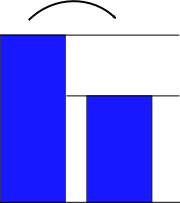
\includegraphics[scale=0.4]{img/pruning.pdf}};
\node (n1) at ( 0.0, 0.85) {$u$};
\node (n2) at ( 0.05, 0.2) {$u'$};
\node (n3) at ( 0.0,-1.0) {$l$};
\node (n4) at (-1.0, 1.5) {pruning by $c_i$};
\node (n5) at (0.8, -0.2) {\large \ldots};
\node (n6) at (6.0, 0.0) {\begin{minipage}{0.7\textwidth}
{\small
\begin{mathpar}
\inferrule{
    \vdots\\
    \inferrule{
        \inferrule{ {} }{ x ∈ [u',u] ∧ c_i \entails ⊥ }{(\thLem)}
    }{
        x ∈ [u',u] ∧ c_i ∧ \bigwedge_{k≠i} c_k \entails ⊥ 
    }{(\weaken)} \\
}{
    x ∈ [l,u] ∧ \bigwedge_k c_k \entails ⊥
}{(\splt)}
\end{mathpar}
}
\end{minipage}
};
\end{tikzpicture}
\caption{Pruning operation and the corresponding proof}
\label{fig:prune}
\end{figure}
